\chapter{Implementation}

% TODO OPT: Note that we had set off to implement it from scratch but were
% working in parallel due to miscommunication?
A skeleton implementation of \viofs{} existed already in \osv{}. % ref https://github.com/cloudius-systems/osv/commit/bae4381d1d0558b7a684294e9203864f9652395c
That included support (via FUSE\_READ) for reading files (but not directories).
In coordination with the members of the \osv{} community, we set out to enhance
it feature-wise. The main focus of this effort was to support reading through
the \viofs{} DAX window, a feature designed and implemented (with
``experimental'' status) by the \viofs{} community with dramatic performance
improvement in mind. Besides that, we had the opportunity to add support for
directory reading as well as booting \osv{} from a \viofs{} root file system.
Over the course of these, other structural changes, fixes and enhancements to
the existing code were necessary.

This chapter details the most significant of these contributions: reading files
using the DAX window and booting off of \viofs{}.

\section{DAX window in \viofs{}}

\osv{}'s internal code structure largely resembles that of most monolithic
kernels, separating the notion of a driver and a file system. Drivers (in
drivers/) are responsible for adhering to an interface that's common across all
members of a particular device family (e.g. block storage or network), allowing
the device to be used by the other kernel subsystems. File systems (in fs/)
also implement a common interface defined by \osv{}'s virtual file system. This
interface encompasses operations such as opening, closing, reading files etc.
Most file systems are implemented over a block device, utilizing its interface
for ``translating'' from high-level file system operations to low-level device
ones. Naturally, there are exceptions to this, like NFS which is backed by the
network subsystem instead.

Virtio-fs is unique in that, as a file system it depends on the corresponding
device which is not part of broader family like block devices. This is of course
FUSE heritage. There is therefore strong, explicit dependence of the \viofs{}
file system from the \viofs{} device driver (fig. \ref{fig:virtiofs-vs-others}),
as is the case on linux, where the two are implemented together (in
fs/fuse/virtio\_fs.c). It is then clear that the distinction between \viofs{}
driver and file system (i.e. partitioning of related functionality) is rather
malleable. Nonetheless, the ensuing presentation is made through the lenses of
this distinction.

\begin{figure}
    \centering
    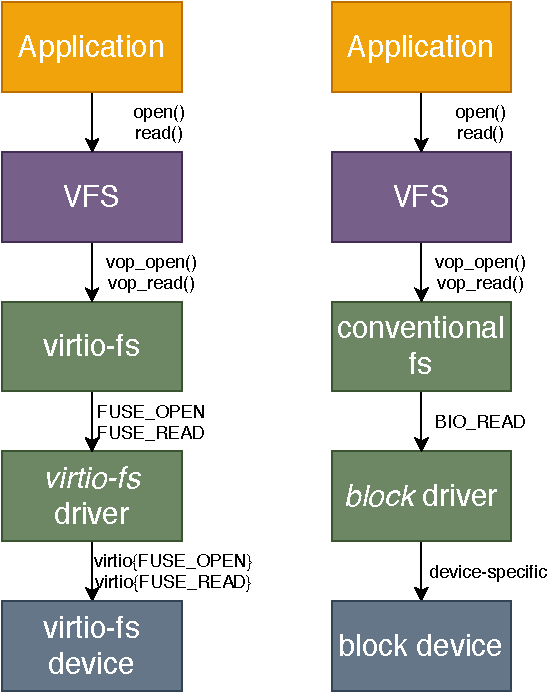
\includegraphics{virtiofs-vs-others}
    \caption{Components and dependencies in the guest: \viofs{} compared to
        conventional local file systems.}
    \label{fig:virtiofs-vs-others}
\end{figure}

\subsection{Driver}

The \viofs{} driver is in charge of direct communication and low-level handling
of the device. Apart from initialization (virtqueue discovery, feature
negotiation) \cite{virtio}, its main task is transferring the requests and
responses to and from the device using the virtqueues. To this end it offers an
asynchronous interface for submitting requests encapsulating FUSE messages. The
driver remains agnostic to FUSE, handling requests as opaque.

The initial \viofs{} implementation in \qemu{} was in the form of a PCI device.
According to the virtio specification \cite{virtio}, the DAX window is the
shared memory region with identifier (``shmid'') 0. In the case of virtio PCI
transport, shared memory regions are realized as PCI BARs (base address
registers), each of which is exposed as a VIRTIO\_PCI\_CAP\_SHARED\_MEMORY\_CFG
PCI capability, having a unique identifier \cite{virtio, wiki:pci-conf,
osdev:pci}.

The first step towards DAX window support was thus to discover it, if offered
by the device. This was almost effortless thanks to \osv{}'s thorough and
well-modeled PCI subsystem. Specifically, it consisted of the following changes:
\begin{enumerate}
    \item Enabling the PCI subsystem to discover multiple capabilities of the
          same type (in drivers/pci-function.cc). This was necessary as,
          previously the discovery functions looked only for the first
          capability of a certain type. This could prove insufficient in the
          case of multiple shared memory regions, which as mentioned above
          correspond to a PCI capability each (although in \viofs{}, currently
          there is only one).
    \item Extending the virtio PCI device model (in
          drivers/virtio-pci-device.cc) so as to discover all the shared memory
          regions of each device, searching for the corresponding capabilities
          and recording the attributes of the BARs those designate.
    \item Extending the \viofs{} device driver (in drivers/virtio-fs.cc) so as
          to discover the shared memory region with id 0 (the DAX window) and
          directly expose it in its interface, as a device MMIO (memory-mapped
          I/O) region. We note that the mapping of the region to the virtual
          address space has already been performed by the device model at this
          point.
\end{enumerate}

\subsection{File system}

The \viofs{} file system assumes a mechanism for communicating FUSE requests
(provided by the driver), building its functionality on top of it. Therefore
it is responsible for the content of the messages the driver simply delivers.

\subsubsection{File mapping}

Mounting a \viofs{} file system consists of opening a FUSE session by sending a
FUSE\_INIT request \cite{virtio}. This carries out the negotiation of the
session parameters, including one concerning the operation of the DAX window:
the map alignment. The first modification required in the file system was thus
to extend the mount process to notify the device of DAX window support in the
OS and collect the parameter's value from the response.

The aforementioned parameter restricts file mappings in the DAX window as per
the following: both the offset of a mapping's start within the file and within
the DAX window must be aligned according to the map alignment. In practice, this
is dictated by the usage of \texttt{mmap()} \cite{man:mmap} on the host, in the
current device implementation (this is also the reason why the map alignment
usually matches the host's page size).

As defined by the specification, providing the DAX window by the device as well
as using it by the guest are both optional. Moreover, DAX window usage is
independent of regular FUSE\_READ usage (which is always available). Our
implementation strives to satisfy all read requests through the DAX window, but
in case that is not available or using it fails, it dynamically switches to the
FUSE\_READ fallback, as seen in fig. \ref{fig:dax-flowchart}.

\begin{lstlisting}[
    float,
    caption=FUSE definitions for the mapping operations. See appendix
        \ref{app:copyright} for copyright notice.,
    label=lst:fuse-defs,
    language=C,
    captionpos=b,
    frame=single,
    basicstyle=\ttfamily,
    commentstyle=\color{olive},
    keywordstyle=\color{blue}]
#define FUSE_SETUPMAPPING_FLAG_WRITE (1ull << 0)
struct fuse_setupmapping_in {
    /* An already open handle */
    uint64_t        fh;
    /* Offset into the file to start the mapping */
    uint64_t        foffset;
    /* Length of mapping required */
    uint64_t        len;
    /* Flags, FUSE_SETUPMAPPING_FLAG_* */
    uint64_t        flags;
    /* memory offset in to dax window */
    uint64_t        moffset;
};

struct fuse_removemapping_in {
    /* number of fuse_removemapping_one follows */
    uint32_t        count;
};

struct fuse_removemapping_one {
    /* Offset into the dax to start the unmapping */
    uint64_t        moffset;
    /* Length of mapping required */
    uint64_t        len;
};
\end{lstlisting}

For establishing a new mapping, \viofs{} extends the FUSE protocol, introducing
the FUSE\_SETUPMAPPING operation. A request of this type is described by a
fuse\_setupmapping\_in struct (the definition can be found in listing
\ref{lst:fuse-defs}). For canceling existing mappings, FUSE\_REMOVEMAPPING has
been introduced, its body consisting of a struct fuse\_removemapping\_in,
followed by the indicated number of fuse\_removemapping\_one structs.

Finally, we note that according to the specification, a new mapping can be
requested which overlaps an existing one. If the overlap is complete, the
existing is replaced by the new one, whereas if it is only partially overlapped,
it is split into smaller mappings. A request for a new mapping may fail in case
of device resource exhaustion, at which point it is recommended to retry the
request after releasing resources by removing existing mappings. Therefore, in
our implementation FUSE\_REMOVEMAPPING is only employed under such exceptional
conditions.

\subsubsection{DAX window manager}

From the fine-grained control over the DAX window mappings arises the problem
of how to manage it optimally. There are a lot in common between this and the
more general problem of memory management in the context of an operating system
with paging, due to the restrictions posed by the map alignment. To tackle this
we came up with a DAX window manager on the file system level, with all read
operations happening through this manager, allowing it to apply the policy
described below.

The management policy was designed with these considerations in mind:
\begin{itemize}
    \item In our case, the file system is read-only.
    \item The time to fulfill a FUSE\_SETUPMAPPING request is independent of the
          mapping's size.
    \item A simpler policy translates to a simpler implementation, which is
          easier to get right and to be performant.
\end{itemize}
According to them, we arrived at a management scheme summarized by the
subsequent characteristics (illustrated in part in fig. \ref{fig:dax-overview}):
\begin{itemize}
    \item The DAX window is split into fixed-size ``chunks'' (1 MiB by default).
          These comprise the building blocks in the sense that all mappings are
          made in terms of these chunks. Every new mapping starts at an offset
          both within the file and within the DAX window, which is a multiple of
          the chunk size and contains an integer amount of chunks. It is then
          apparent that requiring the chunk size to be compatible with the map
          alignment automatically satisfies all the alignment requirements
          placed by the \viofs{} device. This was decided upon, on the one hand
          for simplicity and on the other hand to serve as the unit of
          prefetching (with the right choice of chunk size).
    \item A new mapping always starts from the lowest available address within
          the DAX window. If there is not enough room (the window is full), then
          it overlaps the mappings in the highest addresses, only as much as
          necessary to fit the new one. Hence, a LIFO (Last In - First Out)
          model is applied, with the DAX window resembling a stack. This was
          selected in the name of simplicity as well as to accommodate an
          application reading a file serially in consecutive requests, by having
          consecutive chunks in the file be consecutive in the window too.
    \item No prefetching is done beyond one chunk in order to avoid potential
          waste of space in the DAX window. Nonetheless, we note that the
          implementation support a mode (disabled by default) of ``aggressive''
          prefetching, whereby the whole file is mapped upon the first access to
          it.
\end{itemize}
The whole read process as pertains to the \viofs{} implementation is depicted
in the control flow diagram in fig. \ref{fig:dax-flowchart}.

\begin{figure}
    \centering
    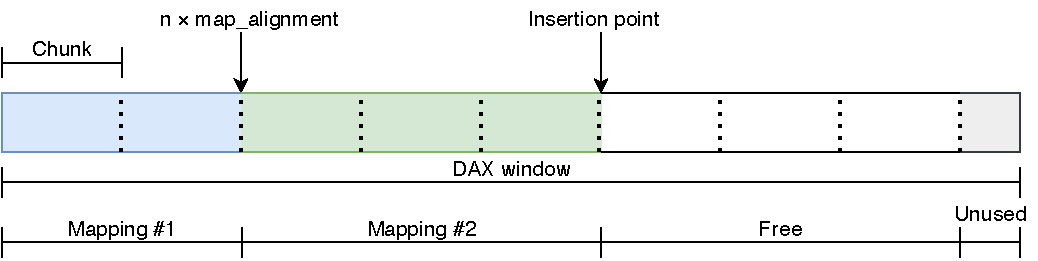
\includegraphics[width=\textwidth]{dax}
    \caption{Indicative view of the DAX window under the manager.}
    \label{fig:dax-overview}
\end{figure}

\begin{figure}
    \begin{minipage}[c][\textheight]{\textwidth}
        \centering
        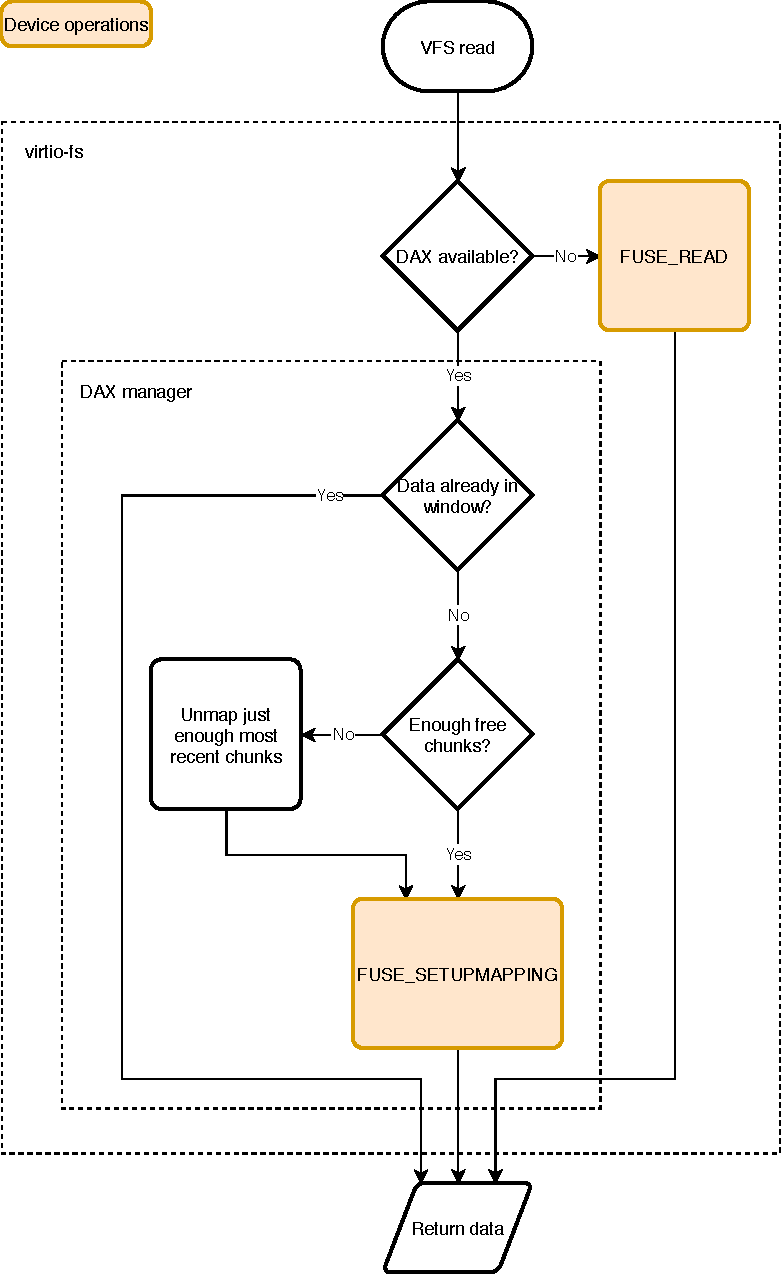
\includegraphics[height=\textheight]{read}
        \caption{Process of reading from \viofs{} under the DAX window manager.}
        \label{fig:dax-flowchart}
    \end{minipage}
\end{figure}

\section{Boot from \viofs{}}

Adding support for booting off of \viofs{} in \osv{} comprised two main
components: the main one concerning the kernel in addition to a supplementary
one having to do with the automation tools for building and running the images.
Both were guided by previous similar extensions, since \osv{} was already able
to use either ZFS or rofs (or even ramfs, as a special case) for its root file
system.

In brief, the points involving the root file system in the lifecycle of an
\osv{} unikernel before our modifications were:
\begin{enumerate}
    \item Building the image (mainly in scripts/build): at this stage the root
          file system type is selected by the user and the root file system is
          built with the contents defined by the application. Moreover, here
          begins the determination of the unikernel's command line, containing
          options for the kernel itself in addition to the command line of the
          application itself. This is stored in a temporary file, where the next
          stage picks it up \cite{osv-wiki:osv-components}.
    \item Executing the image (mainly in scripts/run.py): here the command line
          is optionally complemented with ephemeral options, e.g. the verbosity
          level of the kernel messages. Subsequently the finalized command line
          is written to the image, before that is executed.
    \item Loading the kernel (mainly in loader.cc): following, among others,
          the initialization of the kernel, the devices and drivers and reading
          the command line, \osv{} attempts to transition from its initial,
          embedded file system (ramfs) to the root file system
          \cite{osv-wiki:osv-loader}. This process consists of mounting the file
          system at some point of the existing, initial ramfs, followed by
          pivoting the virtual file system to it. These are made simple thanks
          to the virtual file system, after all prerequisites for its operation
          are completed.
\end{enumerate}
% TODO OPT: Diagram with build / run process and flow of relevant options.

The determination of which file system to use as root during loading was
previously dynamic: there was an attempt to mount the first block device, first
as rofs and, if that failed, as ZFS. If both failed, execution continued with
the initial ramfs file system. Despite the above process being easy to extend to
include \viofs{}, it was clear that there were many silent assumptions, without
allowing much user control. Hence, we decided to go the extra mile and grant
more control over the process: we added a kernel command line option,
\texttt{-{}-rootfs}, which allows explicitly specifying the root file system
type (between ZFS, rofs, \viofs{} and ramfs). As seen in diagram
\ref{fig:rootfs}, this option is optional and, if it is not specified, the
older, dynamic process is adopted, for compatibility. Last, we made the
necessary modifications to the build process (scripts/build) for it set this
option depending on the file system type specified by the user at build time.
Moreover, this way we achieved to make the build process and the available
root file system types more predictable and better documented.

\begin{figure}
    \centering
    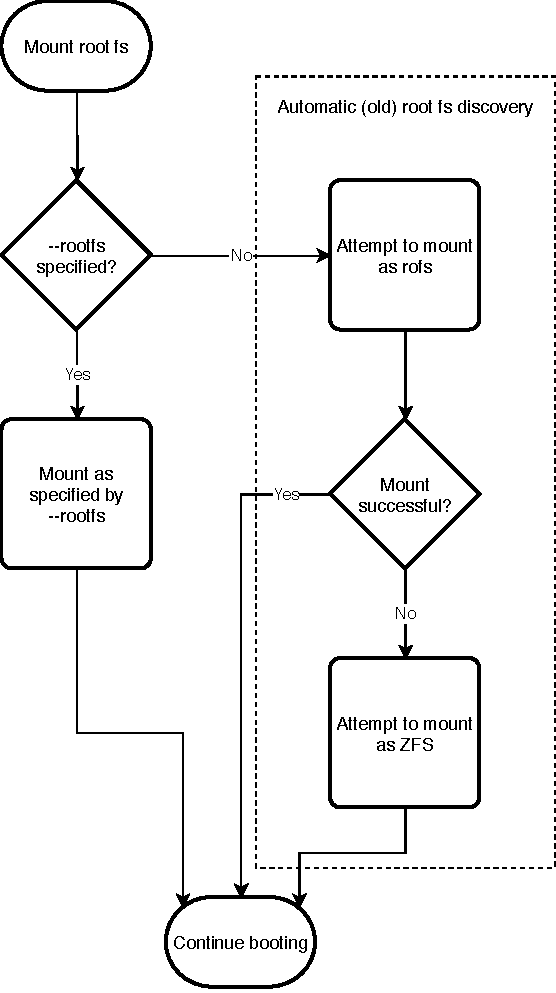
\includegraphics{rootfs}
    \caption{Root file system mounting process.}
    \label{fig:rootfs}
\end{figure}

Finally, as far as \viofs{} itself is concerned, using it as the root file
system did not have any notable challenge in store: if selected via
\texttt{-{}-rootfs}, it was mounted from the first \viofs{} device (in \osv{},
in contrast to linux, those are exposed, serially numbered in the devfs,
instead of being identified by their \viofs{} tag). In order to automatically
populate a directory on the host with the appropriate contents for each
application and Subsequently use that as the \viofs{} shared directory, one can
use the \texttt{export} and \texttt{export\_dir} options to scripts/build.
